% Pascal's theorem: a hexagon inscribed in a conic and its Pascal line.
% Source: book/tex/alg-geom/bezout.tex (§ Application: Pascal's theorem).
\documentclass[border=2mm]{standalone}
\usepackage{tikz}
\begin{document}
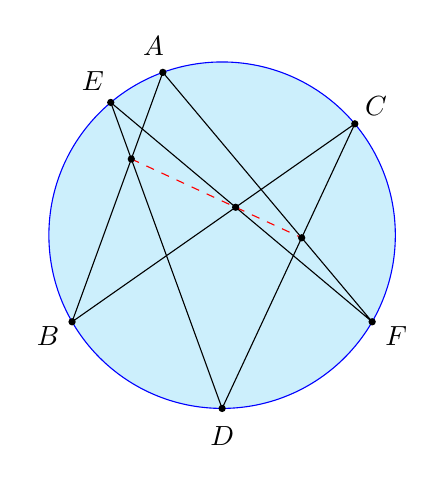
\begin{tikzpicture}[scale=2.2]
  \fill[cyan!20] (0,0) circle (1);
  \draw[blue] (0,0) circle (1);
  \coordinate (A) at (110:1);
  \coordinate (B) at (210:1);
  \coordinate (C) at (40:1);
  \coordinate (D) at (270:1);
  \coordinate (E) at (130:1);
  \coordinate (F) at (-30:1);
  \draw (A)--(B)--(C)--(D)--(E)--(F)--cycle;
  \coordinate (P) at (intersection of A--B and D--E);
  \coordinate (X) at (intersection of B--C and E--F);
  \coordinate (Q) at (intersection of C--D and F--A);
  \draw[red,dashed] (P)--(Q);
  \foreach \p/\d in {A/110,B/210,C/40,D/270,E/130,F/-30}
    {\fill (\p) circle (0.6pt); \node at (\d:1.16) {$\p$};}
  \fill (P) circle (0.6pt); \fill (X) circle (0.6pt); \fill (Q) circle (0.6pt);
\end{tikzpicture}
\end{document}
